\documentclass[aspectratio=169]{beamer}
\usetheme{Madrid}
\usecolortheme{default}

% Packages
\usepackage{amsmath}
\usepackage{amssymb}
\usepackage{graphicx}
\usepackage{tikz}
\usepackage{booktabs}
\usepackage{xcolor}

% Title page information
\title[MCDM for Renewable Energy]{Multi-Criteria Decision Making for Renewable Energy Planning}
\subtitle{Session 1: Fundamentals and Components}
\author{Your Name}
\institute{Your Institution}
\date{\today}

% Custom colors
\definecolor{energygreen}{RGB}{34,139,34}
\definecolor{solarorange}{RGB}{255,140,0}
\definecolor{windblue}{RGB}{70,130,180}

\begin{document}

% Title slide
\begin{frame}
\titlepage
\end{frame}

% Outline
\begin{frame}{Session Overview}
\tableofcontents
\end{frame}

\section{Introduction to MCDM}

\begin{frame}{What is Multi-Criteria Decision Making?}
\begin{block}{Simple Definition}
MCDM helps us choose the best option when we have multiple goals that conflict with each other.
\end{block}

\begin{columns}
\begin{column}{0.6\textwidth}
\textbf{Everyday Example:} Buying a car
\begin{itemize}
\item \textcolor{red}{Low cost} vs. \textcolor{energygreen}{High safety}
\item \textcolor{red}{Fuel efficiency} vs. \textcolor{energygreen}{Performance}
\item \textcolor{red}{Reliability} vs. \textcolor{energygreen}{Style}
\end{itemize}

\vspace{0.3cm}
\textbf{Energy Example:} Choosing power source
\begin{itemize}
\item \textcolor{red}{Cheap} vs. \textcolor{energygreen}{Clean}
\item \textcolor{red}{Reliable} vs. \textcolor{energygreen}{Renewable}
\item \textcolor{red}{Quick to build} vs. \textcolor{energygreen}{Long-term sustainable}
\end{itemize}

\vspace{0.3cm}
\textbf{The Challenge:} No single option is best at everything!
\end{column}
\begin{column}{0.4\textwidth}
\begin{tikzpicture}[scale=0.8]
% Draw a simple decision tree
\node[circle, draw, fill=energygreen!20] (root) at (0,0) {Decision};
\node[rectangle, draw, fill=solarorange!20] (alt1) at (-1.5,-2) {Solar};
\node[rectangle, draw, fill=windblue!20] (alt2) at (0,-2) {Wind};
\node[rectangle, draw, fill=energygreen!20] (alt3) at (1.5,-2) {Hydro};

\draw[->] (root) -- (alt1);
\draw[->] (root) -- (alt2);
\draw[->] (root) -- (alt3);

% Criteria
\node[ellipse, draw, fill=yellow!20] (c1) at (-2,1) {Cost};
\node[ellipse, draw, fill=yellow!20] (c2) at (0,1) {Environment};
\node[ellipse, draw, fill=yellow!20] (c3) at (2,1) {Reliability};

\draw[dashed] (c1) -- (root);
\draw[dashed] (c2) -- (root);
\draw[dashed] (c3) -- (root);
\end{tikzpicture}
\end{column}
\end{columns}
\end{frame}

\begin{frame}{Why MCDM for Renewable Energy?}
\textbf{Energy decisions are especially complex because:}

\begin{columns}
\begin{column}{0.5\textwidth}
\textcolor{energygreen}{\textbf{Multiple Stakeholders:}}
\begin{itemize}
\item Government (policy goals)
\item Utilities (profit, reliability)
\item Communities (jobs, health)
\item Investors (returns)
\item Environmental groups (sustainability)
\end{itemize}

\textcolor{solarorange}{\textbf{Long-term Impact:}}
\begin{itemize}
\item 20-30 year investments
\item Technology changes
\item Climate change effects
\item Policy shifts
\end{itemize}
\end{column}
\begin{column}{0.5\textwidth}
\textcolor{windblue}{\textbf{Multiple Dimensions:}}
\begin{itemize}
\item Economic (cost, jobs)
\item Environmental (emissions, land use)
\item Technical (reliability, efficiency)
\item Social (acceptance, equity)
\end{itemize}

\textcolor{red}{\textbf{High Stakes:}}
\begin{itemize}
\item Billions of dollars
\item Climate targets
\item Energy security
\item Economic development
\end{itemize}
\end{column}
\end{columns}

\vspace{0.3cm}
\begin{center}
\textbf{MCDM provides a systematic way to handle this complexity!}
\end{center>
\end{frame>

\begin{frame}{Real-World Example: Urban Energy Planning}
\begin{block}{Scenario: City of Austin, Texas (Simplified)}
Population 500,000, current demand 800 MW, needs additional 320 MW by 2035. Must reduce CO₂ emissions by 50\% while maintaining reliability and affordability.
\end{block>

\begin{columns}
\begin{column}{0.5\textwidth}
\textbf{Energy Alternatives:}
\begin{itemize}
\item \textcolor{solarorange}{Solar farm} (500 MW, \$600M)
\item \textcolor{windblue}{Wind park} (400 MW, \$800M)
\item Natural gas (320 MW, \$400M)
\item Nuclear (1000 MW, \$8B)
\item Biomass (200 MW, \$300M)
\item Hydro (150 MW, \$500M)
\item Storage + renewables (mixed)
\end{itemize>
\end{column}
\begin{column}{0.5\textwidth}
\textbf{Evaluation Criteria:}
\begin{itemize}
\item Capital cost (\$/MW)
\item Operating cost (\$/MWh)
\item CO₂ emissions (tons/MWh)
\item Reliability (capacity factor \%)
\item Public acceptance (survey 1-10)
\item Job creation (jobs/MW)
\item Land use (acres/MW)
\end{itemize>
\end{column}
\end{columns>

\vspace{0.3cm}
\textcolor{red}{\textbf{The Dilemma:}} Solar is clean but expensive. Gas is cheap but polluting. Nuclear is reliable but controversial. Wind is variable but popular.

\textcolor{energygreen}{\textbf{MCDM Solution:}} Systematic comparison considering ALL factors!
\end{frame>

\begin{frame}{The Problem Without MCDM}
\textbf{What happens when we don't use systematic decision-making?}

\begin{columns}
\begin{column}{0.5\textwidth}
\textcolor{red}{\textbf{Common Problems:}}
\begin{itemize}
\item \textbf{Bias:} Focus on one criterion (usually cost)
\item \textbf{Politics:} Loudest voice wins
\item \textbf{Inconsistency:} Different standards for different options
\item \textbf{Regret:} Overlooked important factors
\item \textbf{Conflict:} Stakeholders fight over priorities
\end{itemize}
\end{column>
\begin{column}{0.5\textwidth}
\textcolor{energygreen}{\textbf{Real Examples:}}
\begin{itemize}
\item Germany's nuclear phase-out (political vs. technical)
\item California's energy crisis (deregulation focus)
\item Texas winter storm (cost vs. reliability)
\item UK wind farms (environment vs. aesthetics)
\end{itemize}
\end{column>
\end{columns>

\vspace{0.5cm}
\begin{center}
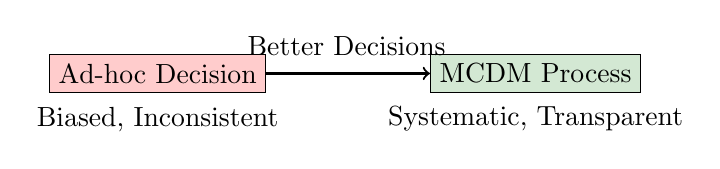
\begin{tikzpicture}[scale=0.8]
% Before and after comparison
\node[rectangle, draw, fill=red!20] (before) at (0,0) {Ad-hoc Decision};
\node[rectangle, draw, fill=energygreen!20] (after) at (6,0) {MCDM Process};

\node[below=0.3cm] at (before) {Biased, Inconsistent};
\node[below=0.3cm] at (after) {Systematic, Transparent};

\draw[thick, ->] (before) -- (after);
\node[above=0.1cm] at (3,0) {Better Decisions};
\end{tikzpicture}
\end{center>
\end{frame>

\section{Components of MCDM}

\begin{frame}{The Five Key Components of MCDM}
\begin{enumerate}
\item \textbf{\textcolor{energygreen}{Defining Alternatives}} - What are our options?
\item \textbf{\textcolor{solarorange}{Establishing Criteria}} - How do we evaluate?
\item \textbf{\textcolor{windblue}{Weighting \& Scoring}} - What matters most?
\item \textbf{\textcolor{red}{Aggregation \& Ranking}} - How do we combine information?
\item \textbf{\textcolor{purple}{Sensitivity Analysis}} - How robust are our results?
\end{enumerate}

\vspace{0.5cm}
\begin{center}
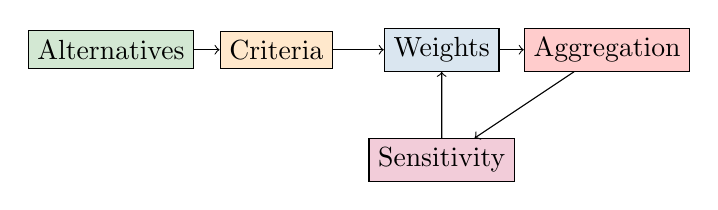
\begin{tikzpicture}[scale=0.7]
% Flow diagram
\node[rectangle, draw, fill=energygreen!20] (alt) at (0,0) {Alternatives};
\node[rectangle, draw, fill=solarorange!20] (crit) at (3,0) {Criteria};
\node[rectangle, draw, fill=windblue!20] (weight) at (6,0) {Weights};
\node[rectangle, draw, fill=red!20] (agg) at (9,0) {Aggregation};
\node[rectangle, draw, fill=purple!20] (sens) at (6,-2) {Sensitivity};

\draw[->] (alt) -- (crit);
\draw[->] (crit) -- (weight);
\draw[->] (weight) -- (agg);
\draw[->] (agg) -- (sens);
\draw[->] (sens) -- (weight);
\end{tikzpicture}
\end{center}
\end{frame}

\begin{frame}{Component 1: Defining Alternatives}
\begin{block}{Definition}
Alternatives are the possible solutions or options we want to compare and choose from.
\end{block}

\textbf{In Renewable Energy Context:}
\begin{itemize}
\item Different types of renewable energy sources
\item Various technology configurations
\item Different scales of implementation
\item Hybrid systems and combinations
\end{itemize}

\vspace{0.3cm}
\begin{columns}
\begin{column}{0.5\textwidth}
\textbf{Example: Rural Electrification}
\begin{itemize}
\item Grid extension
\item Mini-grid solar
\item Solar home systems
\item Micro-hydroelectric
\item Biomass gasification
\item Hybrid renewable system
\end{itemize}
\end{column}
\begin{column}{0.5\textwidth}
\textbf{Key Considerations:}
\begin{itemize}
\item Feasibility and availability
\item Mutual exclusivity
\item Completeness of options
\item Stakeholder preferences
\end{itemize}
\end{column}
\end{columns}
\end{frame}

\begin{frame}{Component 2: Establishing Criteria}
\begin{block}{Definition}
Criteria are the factors we consider in decision-making - the aspects we want to evaluate and optimize.
\end{block}

\textbf{Renewable Energy Criteria Dimensions:}

\begin{columns}
\begin{column}{0.33\textwidth}
\textcolor{energygreen}{\textbf{Economic}}
\begin{itemize}
\item Initial cost (CAPEX)
\item Operating cost (OPEX)
\item Payback period
\item Net present value
\item Job creation
\end{itemize}
\end{column}
\begin{column}{0.33\textwidth}
\textcolor{solarorange}{\textbf{Environmental}}
\begin{itemize}
\item CO₂ emissions
\item Land use impact
\item Water consumption
\item Waste generation
\item Biodiversity impact
\end{itemize}
\end{column}
\begin{column}{0.33\textwidth}
\textcolor{windblue}{\textbf{Technical/Social}}
\begin{itemize}
\item Reliability
\item Efficiency
\item Scalability
\item Public acceptance
\item Energy security
\end{itemize}
\end{column}
\end{columns}

\vspace{0.3cm}
\textbf{Important:} Criteria should be comprehensive, measurable, and non-redundant.
\end{frame}

\begin{frame}{Component 3: Weighting and Scoring}
\begin{columns}
\begin{column}{0.5\textwidth}
\textbf{\textcolor{windblue}{Weighting - "What matters most?"}}
\begin{itemize}
\item Assigns importance to criteria
\item Reflects stakeholder priorities
\item Must sum to 1.0 (100\%)
\end{itemize}

\textbf{Example Weight Scenarios:}
\begin{itemize}
\item \textbf{Utility:} Cost 50\%, Reliability 30\%, Environment 20\%
\item \textbf{Environmental Group:} Environment 60\%, Cost 20\%, Reliability 20\%
\item \textbf{Community:} Jobs 40\%, Cost 30\%, Environment 30\%
\end{itemize}
\end{column}
\begin{column}{0.5\textwidth}
\textbf{\textcolor{solarorange}{Scoring - "How well does each option perform?"}}
\begin{itemize}
\item Rates alternatives on each criterion
\item Can use different scales (1-10, \$, \%, etc.)
\item Should be objective when possible
\end{itemize}

\textbf{Example Scoring:}
\begin{itemize}
\item \textbf{Cost:} \$1200/MW (actual data)
\item \textbf{CO₂:} 0.02 tons/MWh (measured)
\item \textbf{Acceptance:} 7/10 (survey result)
\item \textbf{Reliability:} 35\% (capacity factor)
\end{itemize}
\end{column}
\end{columns}

\vspace{0.3cm}
\textbf{Complete Example:}
\begin{center}
\begin{tabular}{|l|c|c|c|c|}
\hline
\textbf{Criterion} & \textbf{Weight} & \textbf{Solar} & \textbf{Wind} & \textbf{Gas} \\
\hline
Cost (\$/MW) & 0.3 & 1200 & 1600 & 800 \\
CO₂ (tons/MWh) & 0.4 & 0.02 & 0.01 & 0.35 \\
Reliability (\%) & 0.3 & 25 & 35 & 85 \\
\hline
\end{tabular}
\end{center}
\textcolor{blue}{\textbf{Question:}} Which would you choose and why?
\end{frame}

\begin{frame}{Component 4: Aggregation and Ranking}
\begin{block}{Definition}
Aggregation combines scores and weights to calculate overall value. Ranking orders alternatives from best to worst.
\end{block}

\textbf{Common Aggregation Methods:}

\begin{columns}
\begin{column}{0.5\textwidth}
\textbf{Simple Additive Weighting (SAW):}
$$S_i = \sum_{j=1}^{n} w_j \times r_{ij}$$

\textbf{Weighted Product Model (WPM):}
$$P_i = \prod_{j=1}^{n} (r_{ij})^{w_j}$$
\end{column}
\begin{column}{0.5\textwidth}
\textbf{TOPSIS:}
$$C_i = \frac{d_i^-}{d_i^+ + d_i^-}$$

\textbf{AHP:}
$$S_i = \sum_{j=1}^{n} w_j \times w_{ij}$$
\end{column}
\end{columns}

\vspace{0.3cm}
Where:
\begin{itemize}
\item $S_i$ = score for alternative $i$
\item $w_j$ = weight of criterion $j$
\item $r_{ij}$ = normalized score of alternative $i$ on criterion $j$
\end{itemize}
\end{frame}

\begin{frame}{Component 5: Sensitivity Analysis}
\begin{block}{Definition}
Sensitivity analysis tests how changes in weights, scores, or methods affect the final ranking.
\end{block}

\textbf{Why is it important for renewable energy decisions?}
\begin{itemize}
\item Energy planning involves long-term commitments
\item Technology costs and performance change over time
\item Policy priorities may shift
\item Stakeholder preferences may vary
\end{itemize}

\vspace{0.3cm}
\textbf{Types of Sensitivity Analysis:}
\begin{columns}
\begin{column}{0.5\textwidth}
\begin{itemize}
\item \textbf{Weight sensitivity:} How do changes in criterion weights affect ranking?
\item \textbf{Score sensitivity:} How do changes in performance scores affect results?
\end{itemize}
\end{column}
\begin{column}{0.5\textwidth}
\begin{itemize}
\item \textbf{Method sensitivity:} Do different MCDM methods give similar results?
\item \textbf{Scenario analysis:} How do different future scenarios affect decisions?
\end{itemize}
\end{column}
\end{columns}

\vspace{0.3cm}
\textcolor{red}{\textbf{Key Question:}} Are our conclusions robust to reasonable changes in assumptions?
\end{frame}

\section{Case Study Introduction}

\begin{frame}{Case Study: Rural Electrification in Rajasthan, India}
\begin{block}{Real Scenario}
Village cluster with 2,500 households (10,000 people) in Rajasthan. Current: 30\% grid connection, 6 hours/day average supply. Goal: Reliable 16+ hours/day electricity for all households by 2025.
\end{block>

\begin{columns}
\begin{column}{0.5\textwidth}
\textbf{Alternatives with Real Data:}
\begin{enumerate}
\item \textbf{Grid extension:} \$800/household, 12 hrs/day
\item \textbf{Diesel generators:} \$200/household, \$0.25/kWh fuel
\item \textbf{Solar home systems:} \$600/household, 8 hrs/day
\item \textbf{Solar microgrid:} \$1000/household, 18 hrs/day
\end{enumerate}
\end{column}
\begin{column}{0.5\textwidth}
\textbf{Evaluation Criteria:}
\begin{enumerate}
\item \textbf{Cost:} Total 10-year cost per household
\item \textbf{Reliability:} Hours of electricity per day
\item \textbf{Environment:} CO₂ emissions (tons/year)
\item \textbf{Social:} Local job creation (jobs/100 HH)
\item \textbf{Scalability:} Ease of expansion (1-10 scale)
\end{enumerate}
\end{column}
\end{columns}

\vspace{0.3cm}
\textbf{Stakeholder Weights:} Government (cost 40\%, reliability 30\%, environment 20\%, social 10\%)

\textbf{MCDM Result:} Solar microgrid wins despite higher upfront cost!

\textcolor{blue}{\textbf{Session 2:}} We'll calculate this step-by-step and see why!
\end{frame}

\section{Preparation for Group Work}

\begin{frame}{Afternoon Group Work Preview}
\textbf{Group Activity:} Each group will tackle a different renewable energy planning problem

\begin{columns}
\begin{column}{0.5\textwidth}
\textbf{Available Problems:}
\begin{enumerate}
\item Regional energy planning (city scale)
\item Campus energy planning (university)
\item Rural electrification planning
\item Industrial energy selection
\item Residential energy systems
\item Community energy projects
\end{enumerate}
\end{column}
\begin{column}{0.5\textwidth}
\textbf{Group Tasks:}
\begin{enumerate}
\item Define the problem context
\item Identify alternatives and criteria
\item Assign weights (group consensus)
\item Apply MCDM method
\item Perform sensitivity analysis
\item Present recommendations
\end{enumerate}
\end{column}
\end{columns}

\vspace{0.3cm}
\textbf{Tools Available:}
\begin{itemize}
\item Interactive MCDM Learning Tool (web-based)
\item Excel templates
\item Pre-loaded example problems
\end{itemize}

\textcolor{red}{\textbf{Think about:}} What renewable energy challenges interest your group most?
\end{frame}

\begin{frame}{Session 1 Summary}
\textbf{Key Takeaways:}
\begin{enumerate}
\item MCDM provides a systematic approach to complex energy decisions
\item Five key components: Alternatives, Criteria, Weighting/Scoring, Aggregation, Sensitivity
\item Renewable energy decisions involve economic, environmental, and social trade-offs
\item Sensitivity analysis is crucial for robust decision-making
\end{enumerate}

\vspace{0.5cm}
\textbf{Coming Up:}
\begin{itemize}
\item \textbf{Session 2:} MCDM Methods and Techniques (SAW, WPM, TOPSIS, AHP)
\item \textbf{Session 3:} Advanced Applications and Implementation
\item \textbf{Afternoon:} Hands-on group work with real energy problems
\end{itemize}

\vspace{0.5cm}
\begin{center}
\textcolor{energygreen}{\Large Questions?}
\end{center}
\end{frame}

\end{document}
